\section{Exercise 1} \label{P1}
% Write some intro
\textit{[Comment] For the last exercises include an image of the initial robot image of the final robot configuration} 

\textit{[Comment] For each exercise report the results obtained and provide an explanation of the result obtained (even though it might seem trivial). The matlab code is NOT an explanation of the algorithm.} 

\subsection*{Q1.1}
Given the ease of representation and comprehension of serial chain pose, it is crucial to compute the transformation matrices for each joint with respect to the preceding one. For instance, the transformation matrices $^i_jT_0$ in the initial configuration ($\mathbf{q}_0 = \mathbf{q} = \mathbf{0}_{1 \times 7}$) represent the transformation from frame $<i>$ with respect to the next consecutive frame $<j>$. It takes into account both the rotational and translational contributions:
\begin{itemize}
	\item The rotational contribution is computed with \textit{Yaw-Pitch-Roll} convention for rotation, which defines the sequence of rotations around the $z$, $y$, and $x$ axes, respectively;
	\item The translational contribution is represented by the elements contained in the first three rows of the last column of the transformation matrix.
\end{itemize}
It’s crucial to emphasize that these matrices vary based on the values of the vector $\mathbf{q}$ that contain values for uniquely determining each joint’s configuration.
Given the general form of the transformation matrix:
\begin{equation}
	^i_j T = \begin{pmatrix}
		^i_j R & ^i_j P \\
		\mathbf{0}_{1\times3} & 1
	\end{pmatrix}
\end{equation}
where $j$ is the considered chain's joint and $i$ is the joint with respect is considered the transformation, $^i_j R$ is the rotation matrix that define the rotation from the frame $<i>$ to $<j>$, and $^i_j P$ is the position of the frame $<j>$ with respect to frame $<i>$.
Taking into account $\mathbf{q} = \mathbf{0}_{1 \times 7}$ the transformation matrixes for the initial configuration of the chain are:
\begin{align*}
	% Transformation matrix b to 1
	&^b_1 T_0 = \begin{pmatrix}
		1 & 0 & 0 & 0 \\
		0      & 1 & 0 & 0 \\
		0      & 0 & 1 & 0.105 \\
		0      & 0 & 0 & 1
	\end{pmatrix} \quad
	% Transformation matrix 1 to 2
	^1_2 T_0 = \begin{pmatrix}
		0 & 1 & 0 & 0 \\
		0 & 0 & 1 & 0 \\
		1 & 0 & 0 & 0.110 \\
		0 & 0 & 0 & 1
	\end{pmatrix} \quad
	% Transformation matrix 2 to 3
	^2_3 T_0 = \begin{pmatrix}
		0 & 0 & 1 & 0.100 \\
		0 & -1 & 0 & 0 \\
		1 & 0 & 0 & 0 \\
		0 & 0 & 0 & 1
	\end{pmatrix} \quad
	% Transformation matrix 3 to 4
	^3_4 T_0 = \begin{pmatrix}
		0 & 0 & 1 & 0 \\
		0 & -1 & 0 & 0 \\
		1 & 0 & 0 & 0.325 \\
		0 & 0 & 0 & 1
	\end{pmatrix}
	\\
	% Transformation matrix 4 to 5
	&^4_5 T_0 = \begin{pmatrix}
		0 & 0 & 1 & 0.095 \\
		-1 & 0 & 0 & 0\\
		0 & -1 & 0 & 0\\
		0 & 0 & 0 & 1
	\end{pmatrix} \quad 
	% Transformation matrix 5 to 6
	^5_6 T_0 = \begin{pmatrix}
		-1 & 0 & 0 & 0 \\
		0 & -1 & 0 & 0 \\
		0 & 0 & 1 & 0.095 \\
		0 & 0 & 0 & 1
	\end{pmatrix} \quad
	% Transformation matrix 6 to e
	^6_e T_0 = \begin{pmatrix}
		1 & 0 & 0 & 0 \\
		0 & 1 & 0 & 0 \\
		0 & 0 & 1 & 0.355 \\
		0 & 0 & 0 & 1
	\end{pmatrix}
\end{align*}

where:
\begin{itemize}
	\item $^b_1 T_0$ describes solely a translation along the $x$ axis of $0.105\,m$, then $^b_1 \mathbf R_0 = \mathbf I_{3 \times 3}$ and $^b_1 \mathbf P = (0,\,0,\,0.105)^T$;
	\item $^1_2 T_0$ represents two $\frac{\pi}{2}$ rotations, one around $z$ and one other around $y$, both clockwise. There is also a translation component along the $z$ axis of $0.110\,m$, then $^1_2 \mathbf R_0 = \mathbf R_z(-\frac{\pi}{2}) \cdot \mathbf R_y(-\frac{\pi}{2})$ and $^1_2 \mathbf P = (0,\,0,\,0.110)^T$;
	\item $^2_3 T_0$, as $^1_2 T_0$, has two clockwise rotations around $z$ of $\pi$ and $y$ of $\frac{\pi}{2}$ and a translation along $x$ of $0.100\,m$. Formally it means $^2_3 \mathbf R_0 = \mathbf R_z(-\pi) \cdot \mathbf R_y(-\frac{\pi}{2})$ and $^2_3 \mathbf P = (0.100,\,0,\,0)^T$;
	\item $^3_4 T_0$ describes an counterclockwise rotations around $z$ of $\pi$ and a clockwise rotation$y$ of $\frac{\pi}{2}$ and a translation along $z$ of $0.325\,m$. Formally it means $^3_4 \mathbf R_0 = \mathbf R_z(\pi) \cdot \mathbf R_y(-\frac{\pi}{2})$ and $^3_4 \mathbf P = (0,\,0,\,0.325)^T$;
	\item $^4_5 T_0$ represents two clockwise rotations around $z$ and $x$ of $\frac{\pi}{2}$ and a translation along $x$ of $0.325\,m$. Formally it means $^4_5 \mathbf R_0 = \mathbf R_z(-\frac{\pi}{2}) \cdot \mathbf R_y(-\frac{\pi}{2})$ and $^4_5 \mathbf P = (0.095,\,0,\,0)^T$;
	\item $^5_6 T_0$ express a counterclockwise rotation around $z$ of $\pi$ and a translation along $z$ of $0.095\,m$. Then $^5_6 \mathbf R_0 = \mathbf R_z(\pi)$ and $^5_6 \mathbf P = (0,\,0,\,0.095)^T$;
	\item $^6_e T_0$ highlight the presence of a translation along $z$ of $0.335\,m$. Then $^6_e \mathbf R_0 = \mathbf I_{3 \times 3}$ and $^6_e \mathbf P = (0,\,0,\,0.335)^T$.
\end{itemize}

\subsection*{Q1.2}
When the chain's pose changes a good method to update the initial configuration is through the transformation matrix:
\begin{equation*}
	{}^i_j T = {}^i_j T_0 \cdot T_{\text{joint},j}
\end{equation*}
where $^i_j T$ is defined as the transformation matrix for the new pose, and $T_{\text{joint},j}$ is the transformation matrix that accounts for the joint’s change of configuration, define as:
\begin{equation*}
	T_{\text{joint},j} = \begin{pmatrix}
		R_{z}(q_{j}) & P_{z}(q_{j}) \\
		\mathbf{0_{1x3}} & 1
	\end{pmatrix}
\end{equation*}
where joint $j$, because the $z$ axis is defined coinciding with the joint's rotation axis, can either rotates according to $R_{z}(q_{j})$ or traslates by $P_{z}(q_{j})$. If there is:
	\begin{itemize}
		\item a rotational joint: only the rotational part of the transformation matrix contribute to the new configuration. The rotation is along along the $z$-axis and the new $T_{\text{joint},j}$ is:
		\begin{equation*}
			T_{\text{joint},j} = \begin{pmatrix}
				\cos(q) & -\sin(q) & 0 & 0 \\
				\sin(q) & \cos(q) & 0 & 0 \\
				0 & 0 & 1 & 0 \\
				0 & 0 & 0 & 1 \\
			\end{pmatrix} 
		\end{equation*}
		\item a traslational joint: in this case, there is only a translation along the $z$-axis, then $T_{\text{joint},j}$ becomes:
		\begin{equation*}
		T_{\text{joint},j} = \begin{pmatrix}
			1 & 0 & 0 & 0 \\
			0 & 1 & 0 & 0 \\
			0 & 0 & 1 & q \\
			0 & 0 & 0 & 1 \\
		\end{pmatrix} 
		\end{equation*}
	\end{itemize}
For istance, if the vector is $\mathbf{q} = (pi/4, -pi/4, 0, -pi/4, 0, 0.15, pi/4)$, the updeted trasformation matrix are: 
\begin{gather*}
	^b_1 T(q_{t}) = \begin{pmatrix}
		0.7071 & -0.7071 & 0 & 0 \\
		0.7071 & 0.7071 & 0 & 0 \\
		0 & 0 & 1.0000 & 0.1050 \\
		0 & 0 & 0 & 1.0000
	\end{pmatrix} \quad
	^1_2 T(q_{t}) = \begin{pmatrix}
		-0.7071 & 0.7071 & 0 & 0 \\
		0 & 0 & 1.0000 & 0 \\
		0.7071 & 0.7071 & 0 & 0.1100 \\
		0 & 0 & 0 & 1.0000
	\end{pmatrix} \\
	\\
	\quad ^2_3 T(q_{t}) = \begin{pmatrix}
		0 & 0 & 1.0000 & 0.1000 \\
		0 & -1.0000 & 0 & 0 \\
		1.0000 & 0 & 0 & 0 \\
		0 & 0 & 0 & 1.0000
	\end{pmatrix} \quad
	^3_4 T(q_{t}) = \begin{pmatrix}
		0 & 0 & 1.0000 & 0 \\
		0.7071 & -0.7071 & 0 & 0 \\
		0.7071 & 0.7071 & 0 & 0.3250 \\
		0 & 0 & 0 & 1.0000
	\end{pmatrix} \quad \\
	\\
	\quad \quad ^4_5 T(q_{t}) = \begin{pmatrix}
		0 & 0 & 1.0000 & 0.0950 \\
		-1.0000 & 0 & 0 & 0 \\
		0 & -1.0000 & 0 & 0 \\
		0 & 0 & 0 & 1.0000
	\end{pmatrix} \quad
	^5_6 T(q_{t}) = \begin{pmatrix}
		-1.0000 & 0 & 0 & 0 \\
		0 & -1.0000 & 0 & 0 \\
		0 & -0 & 1.0000 & 0.2450 \\
		0 & 0 & 0 & 1.0000
	\end{pmatrix} \quad \\
	\\
	^6_7 T(q_{t}) = \begin{pmatrix}
		0.7071 & -0.7071 & 0 & 0 \\
		0.7071 & 0.7071 & 0 & 0 \\
		0 & 0 & 1.0000 & 0.355 \\
		0 & 0 & 0 & 1.0000
	\end{pmatrix} \quad
	\nonumber
\end{gather*}
\begin{itemize}
	\item $^b_1 T(q_{t})$: in this case, the value of $q$ is $\frac{\pi}{4}$, so there is only a rotation around the $z$-axis. The result can be verified by comparing the new matrix $^1_b T(q_{t})$ with $^b_1 T_{0}$ calculated in exercise 1. It is evident that there is a variation only in the $R_{z}(q)$ component, while $P_{z}(q)$ remains unchanged.
	\item $^1_2 T(q_{t})$: for this configuration, the value of $q$ is $-\frac{\pi}{4}$. As in the previous case, only $R_{z}(q)$ contributes to the new configuration, while the traslational part remains unchanged. The value present in the last column derives from the initial configuration.
	\item $^2_3 T(q_{t})$: in this case, since $q$ is zero, the configuration remains unchanged. It is evident that $^2_3 T(q_{t}) = \,^2_3 T_{0}$. 
	\item $^3_4 T(q_{t})$: the value of $q$ in this configuration is $-\frac{\pi}{4}$. As a result, there is only a rotational contribution along the $z$-axis and no translation.
	\item $^4_5 T(q_{t})$: the value of $q$, as in the case of $^2_3 T(q_{t})$, is zero. Therefore, no rotations or variations occur. The resulting matrix is equivalent to the initial matrix, $^4_5 T_{0}$.
	\item $^5_6 T(q_{t})$: this configuration is characterized by a translational contribution, with $q$ equal to 0.15. The matrix remains unchanged from the initial configuration in terms of the rotational component, while $P_{z}(q)$ is affected by the traslation along the $z$-axis.
	\item $^6_7 T(q_{t})$: in the final configuration, the value of $q$ is $\frac{\pi}{4}$, corresponding to a rotation around the $z$-axis. This means that the translational part, $P_{z}(q)$, remains unchanged. As a result, the new transformation matrix $^6_7 T(q_{t})$ will differ from the initial configuration matrix $^6_7 T_{0}$ only in its rotational component, specifically in the elements of the $R_{z}$ sub-matrix that encode the rotation about the $z$-axis.
\end{itemize}
\subsection*{Q1.3}
For this part of the assignment, we used the following equation to compute the transformation matrix from the base to a given frame:
\begin{equation*}
	^i_e T = \prod_{i=1}^{e} {}^{i-1}_{i} T 
\end{equation*}
The task required computing the transformation matrices for two different configurations:
\begin{equation*}
		^b_e T = \begin{pmatrix}
		-0.5000 & -0.5000 & -0.7071 & -0.7039\\
		0.5000 & 0.5000 & -0.7071 & -0.7039 \\
		0.7071 & -0.7071 & 0.0000 & 0.5155 \\
		0 & 0 & 0 & 1.0000 \\
		\end{pmatrix}
\end{equation*}
This matrix describe the final configuration of the manipulator after the simulation. The traslational's result along $z$ axes can be verified with Fig.\ref{fig:finalconfiguration_z}: it is evident that the total traslation is $0.5155$ metres; while the Fig.\ref{fig:finalconfiguration_xy} display the traslation's result, along $y$ and $x$ with the same value of $-0.7039$.%ripetere contributo rot????\\
\\	$^5_3 T$ =

\subsection*{Q1.4}
In the last exercise, it is required to compute the Jacobian matrix of a manipulator for the end-effector, based on a given geometric model. \\
The basic Jacobian matrix, which consists of two components: an angular contribution matrix $^b J^A_{e}$, and a linear contribution matrix $^b J^L_{e/b}$.
The basic Jacobian is expressed as:
	\begin{equation*}
		\renewcommand{\arraystretch}{1.5}
		^b J_{e/b} = \begin{pmatrix}
			^b J^A_{e} \\ 
			^b J^L_{e/b}
		\end{pmatrix}
	\end{equation*}
	These contributions are computed based on the type of joint (prismatic or rotational) considered, using the following relationships:
	\begin{equation}
		\begin{array}{l}
			\text{Rotational joint}\\ 
			\text{Prismatic joint} \quad 
		\end{array} {}
		^bJ_{e}^A =
		\begin{cases}
			k_{z} \\
			\mathbf{0}
		\end{cases} {}
		^bJ_{e/b}^L =
		\begin{cases}
			k_{z} \times r_{e/b} \\
			k_{z} 
		\end{cases}
	\end{equation}
	where $\mathbf{k_{z}}$ is the unit vector along the joint axis, and $r_{e/b}$ is the position vector from the base to the end-effector.
We obtain the Jacobian for the manipulator’s end-effector, which reflects both the joint
 contributions and the rigid-body effects:
\begin{equation*} 
	^b J_{e/b} = \begin{pmatrix}
		0 & 0 & 0 & 0 & 0 & 0 & 0\\
		0 & 0 & 0 & 0 & 0 & 0 & 0\\
		1.0000 & 1.0000 & 1.0000 & 1.0000 & 1.0000 & 0 & 1.0000 \\ 
		0 & 0 & 0.0500 & 0.2125 & 0.2797 & 0 & 0.7039 \\
		0 & 0 & -0.0500 & -0.2125 & -0.2797 & 0 & -0.7039 \\
		0 & 0 & 0 & 0 & 0 & 1.0000 & 0\\
	\end{pmatrix}	 
\end{equation*}
\begin{figure}[h] 
	\centering
	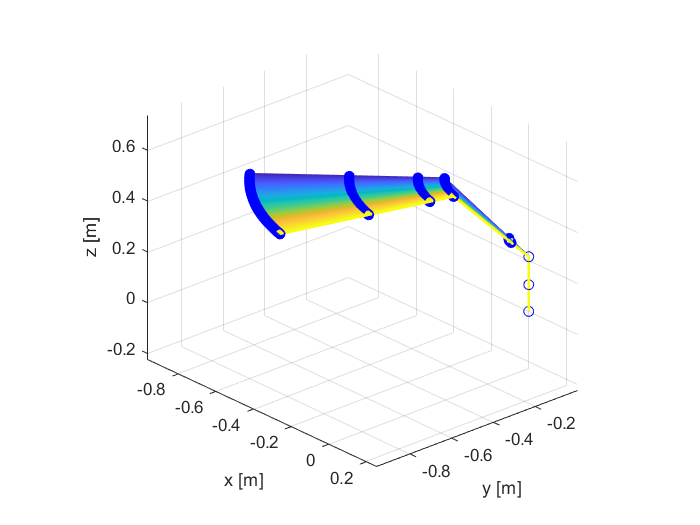
\includegraphics[width=0.9\linewidth]{MotionOfTheManipulator}
	\caption{Descritpion of the manipulator's motion with a 3 dimentional graph. $x$ and $y$ are horizontal axis, while $z$ is vertical axes. Measurement's unit for the three axis is meters.}
	\label{fig:motionofthemanipulator}
\end{figure}
\begin{figure}[h] 
	\centering
	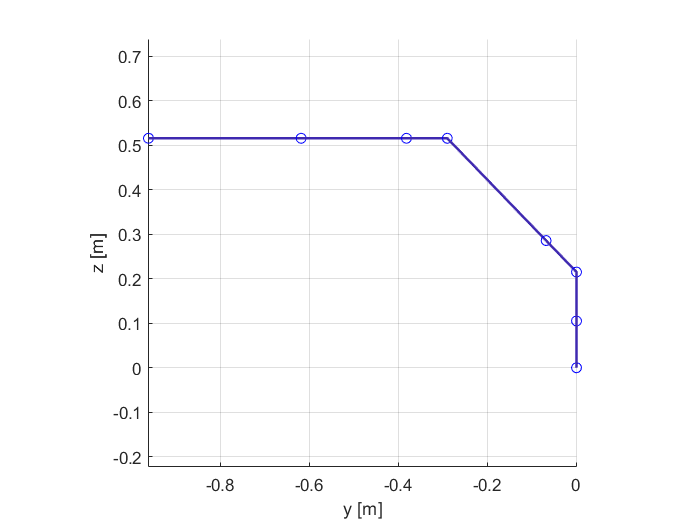
\includegraphics[width=0.9\linewidth]{FinalConfiguration}
	\caption{Configuration of the manipulator at the simulation's end. Measurement's unit for each axis is meters.}
	\label{fig:finalconfiguration_z}
\end{figure}
\begin{figure}[h] 
	\centering
	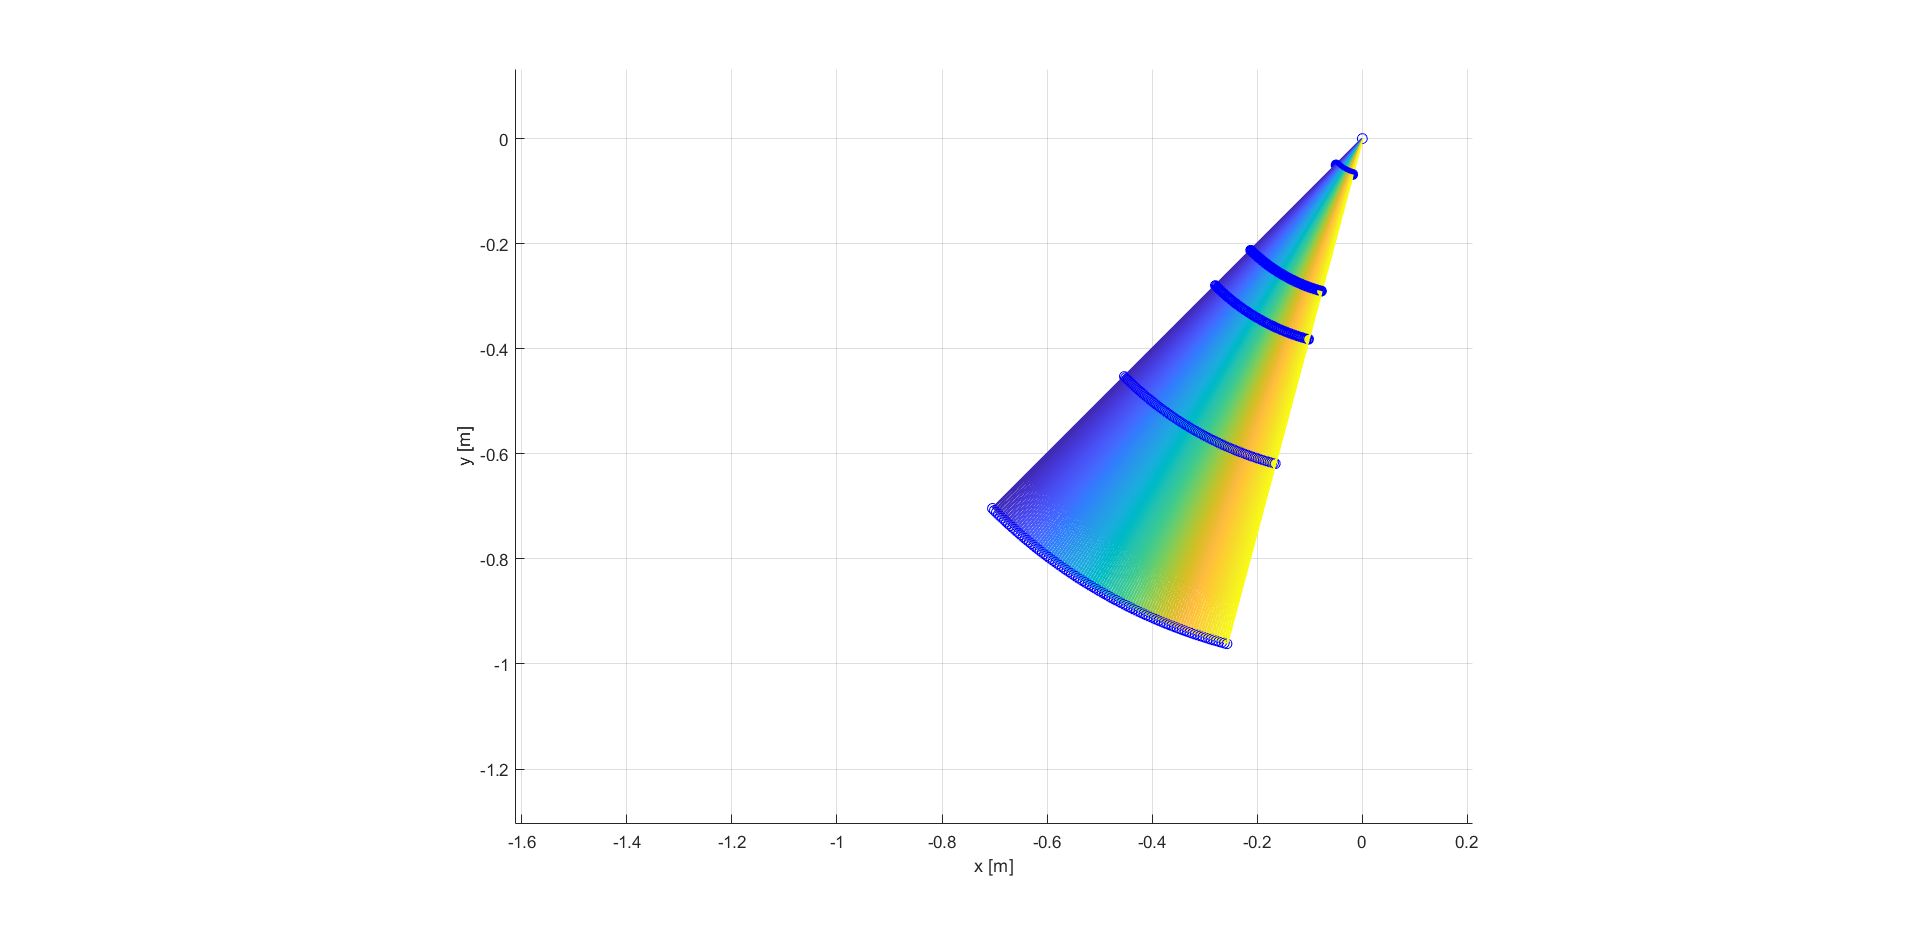
\includegraphics[width=0.95\linewidth]{MotionOfTheManipulator_xy}
	\caption{Fig.\ref{fig:motionofthemanipulator} on plane $xy$}
	\label{fig:finalconfiguration_xy}
\end{figure}

% Q1.1: notazione pedici P
% modifica axis e axes
% \pi in Q1.2
